
\documentclass[journal]{vgtc}                % final (journal style)
%\documentclass[review,journal]{vgtc}         % review (journal style)
%\documentclass[widereview]{vgtc}             % wide-spaced review
%\documentclass[preprint,journal]{vgtc}       % preprint (journal style)
%\documentclass[electronic,journal]{vgtc}     % electronic version, journal

%% Uncomment one of the lines above depending on where your paper is
%% in the conference process. ``review'' and ``widereview'' are for review
%% submission, ``preprint'' is for pre-publication, and the final version
%% doesn't use a specific qualifier. Further, ``electronic'' includes
%% hyperreferences for more convenient online viewing.

%% Please use one of the ``review'' options in combination with the
%% assigned online id (see below) ONLY if your paper uses a double blind
%% review process. Some conferences, like IEEE Vis and InfoVis, have NOT
%% in the past.

%% Please note that the use of figures other than the optional teaser is not permitted on the first page
%% of the journal version.  Figures should begin on the second page and be
%% in CMYK or Grey scale format, otherwise, colour shifting may occur
%% during the printing process.  Papers submitted with figures other than the optional teaser on the
%% first page will be refused.

%% These three lines bring in essential packages: ``mathptmx'' for Type 1
%% typefaces, ``graphicx'' for inclusion of EPS figures. and ``times''
%% for proper handling of the times font family.

\usepackage{mathptmx}
\usepackage{graphicx}
\usepackage{times}
\usepackage{booktabs}
\usepackage{float}

%% We encourage the use of mathptmx for consistent usage of times font
%% throughout the proceedings. However, if you encounter conflicts
%% with other math-related packages, you may want to disable it.

%% This turns references into clickable hyperlinks.
\usepackage[bookmarks,backref=true,linkcolor=black]{hyperref} %,colorlinks
\hypersetup{
  pdfauthor = {},
  pdftitle = {},
  pdfsubject = {},
  pdfkeywords = {},
  colorlinks=true,
  linkcolor= black,
  citecolor= black,
  pageanchor=true,
  urlcolor = black,
  plainpages = false,
  linktocpage
}

%% If you are submitting a paper to a conference for review with a double
%% blind reviewing process, please replace the value ``0'' below with your
%% OnlineID. Otherwise, you may safely leave it at ``0''.
\onlineid{0}

%% declare the category of your paper, only shown in review mode
\vgtccategory{Research}

%% allow for this line if you want the electronic option to work properly
\vgtcinsertpkg

%% In preprint mode you may define your own headline.
%\preprinttext{To appear in IEEE Transactions on Visualization and Computer Graphics.}

%% Paper title.

\title{Visualizing the TDD Cycle}

%% This is how authors are specified in the journal style

%% indicate IEEE Member or Student Member in form indicated below
\author{Michael Hilton, Mihai Codoban, and Caius Brindescu}
\authorfooter{
%% insert punctuation at end of each item
\item
 Michael Hilton is with OSU. E-mail: hiltonm@eecs.oregonstate.edu.
\item
 Mihai Codoban is with OSU. E-mail: codobanm@eecs.oregonstate.edu.
\item
 Caius Brindescu is with OSU. E-mail: brindesc@eecs.oregonstate.edu.
}

%other entries to be set up for journal
%\shortauthortitle{Biv \MakeLowercase{\textit{et al.}}: Global Illumination for Fun and Profit}
%\shortauthortitle{Firstauthor \MakeLowercase{\textit{et al.}}: Paper Title}

%% Abstract section.
%\abstract{
%} % end of abstract

%% Keywords that describe your work. Will show as 'Index Terms' in journal
%% please capitalize first letter and insert punctuation after last keyword
%\keywords{Radiosity, global illumination, constant time}

%% ACM Computing Classification System (CCS). 
%% See <http://www.acm.org/class/1998/> for details.
%% The ``\CCScat'' command takes four arguments.

%\CCScatlist{ % not used in journal version
 %\CCScat{K.6.1}{Management of Computing and Information Systems}%%
%{Project and People Management}{Life Cycle};
% \CCScat{K.7.m}{The Computing Profession}{Miscellaneous}{Ethics}
%}

%% Uncomment below to include a teaser figure.
%   \teaser{
%   \centering
%   \includegraphics[width=16cm]{CypressView}
%   \caption{In the Clouds: Vancouver from Cypress Mountain.}
%  }

%% Uncomment below to disable the manuscript note
%\renewcommand{\manuscriptnotetxt}{}

%% Copyright space is enabled by default as required by guidelines.
%% It is disabled by the 'review' option or via the following command:
% \nocopyrightspace

%%%%%%%%%%%%%%%%%%%%%%%%%%%%%%%%%%%%%%%%%%%%%%%%%%%%%%%%%%%%%%%%
%%%%%%%%%%%%%%%%%%%%%% START OF THE PAPER %%%%%%%%%%%%%%%%%%%%%%
%%%%%%%%%%%%%%%%%%%%%%%%%%%%%%%%%%%%%%%%%%%%%%%%%%%%%%%%%%%%%%%%%

\begin{document}

%% The ``\maketitle'' command must be the first command after the
%% ``\begin{document}'' command. It prepares and prints the title block.

%% the only exception to this rule is the \firstsection command
\firstsection{Introduction}

\maketitle

%% \section{Introduction} %for journal use above \firstsection{..} instead

Software processes have had little or no visualization aids.
Without this kind of information, it is hard to grasp whether these processes are followed correctly. It is hard to find anomalies, and identify potential areas for improvement. Without visualizations that show the big picture, one has to go through tedious, time consuming and incomplete data to learn how a processes was actually implemented. One has to go through reports, interviews and mine software artefacts in order to gain a big picture understanding on how a particular team implemented a software process.

We intend to build visualizations that aid in analyzing developers' TDD practice. Such visualizations would visually expose, for each developer, the main stages of the practice and how they evolve over time.

This kind of information benefits developers, managers and researchers. Developers can better improve their practice by analyzing their past behaviour. Managers can get a sense of magnitude of how well TDD is implemented in the team. Researchers can gain insights and better describe the theoretical foundations of TDD by finding patterns and exploring the divide between practical and theoretical TDD.

\section{Target Audience/User}

The target audience for this visualization is anyone who wants to know about how the software development process happened.  

Developers who want to analyze their own TDD cycle can use this visualization to examine their performance and look for ways to improve their practice.

Researchers analyzing the practice of TDD can use this to look for patterns in how TDD is actually used.  Without this visualization, the data would be a series of JSON files that would be almost impossible to get meaning from just by looking at them.  

Finally, managers analyzing the performance of those that they are managing can use this visualization to have an accurate picture of their team's performance.

\section{High level domain question/questions of interest}
\label{sec:highq}

\textbf{Developers:} \\
Q1: What does my TDD workflow look like? \\
Q2: How does my TDD workflow compare to others'? \\
Q3: How does my TDD workflow change over time? \\

\textbf{Managers:} \\
Q1: How consistent are my developers in using TDD? \\
Q2: Who are the best TDD performers? \\

\textbf{Researchers:} \\
Q1: What does a practica l TDD workflow look like? \\
Q2: How does practical TDD differ from theoretical TDD? \\

\section{Detailed questions that users may ask of the data}

\textbf{Developers:}

Q1: What does my TDD workflow look like? 
\begin{itemize}
	\item What part of the TDD cycle to I spend the most time in?
	\item What part of the TDD cycle do I write the most code in?
	\item How close does my workflow compare with ideal TDD?
	\item What code did I write for a specific TDD stage?
\end{itemize}

Q2: How does my TDD workflow compare to others'?
\begin{itemize}
	\item How does the time I spend in each TDD cycle compare to others?
	\item How does the code I write in each TDD cycle compare to others?
	\item How close is my workflow to the ideal TDD in comparison with others?
\end{itemize}

Q3: How does my TDD workflow change over time?
\begin{itemize}
	\item Is my TDD workflow consistent?
	\item How does the time I spend in each TDD cycle change over time?
	\item How does the amount of code I write in each TDD cycle change over time?
\end{itemize}

\noindent\textbf{Managers:} 

Q1: How consistent are my developers in using TDD?
\begin{itemize}
	\item How much time does each developer spend in each TDD cycle?
	\item How much code does each developer write in each TDD cycle?
	\item How much time do all developers spend in each TDD cycle on average?
	\item How much code do all developers write in each TDD cycle on average?
	\item What percentage of the code my developers write conforms to the TDD model?
\end{itemize}

Q2: Who are the best TDD performers? 
\begin{itemize}
	\item Which developers have a process that is closest to the ideal TDD process?
	\item Which developers spend the least/most time in each TDD cycle?
	\item Which developers write the least/most code in each TDD cycle?
\end{itemize}
	
\noindent\textbf{Researchers:}

Q1: What does a practical TDD workflow look like?
\begin{itemize}
	\item How much time do TDD developers spend in each TDD cycle?
	\item How much code do TDD developers write in each TDD cycle?
	\item What percentage of code that developers write follows the ideal TDD model?
\end{itemize}
	
Q2: How does practical TDD differ from theoretical TDD?
\begin{itemize}
	\item What are patterns that we can identify in how developers write using the TDD process?
	\item How does the time TDD developers spend in each cycle compare with our reference implementation of the TDD process?
	\item How does the code TDD developers write in each cycle compare with our reference implementation of the TDD process?
\end{itemize}

\section{Abstract operations/tasks that must be supported in order to answer the detailed questions
}

Compute TDD cycles: starting from low level text edits, cluster the edits according to the TDD cycle stages: red, green, blue. \\
 
\noindent\textbf{DQ1a:} Compute TDD cycles. Compare cycle stage times \\
\textbf{DQ1b:} Compute TDD cycles. Compare cycle stage size \\
\textbf{DQ1c:} Compute TDD cycles. Retrieve ideal TDD cycles. Compare user cycles and style with theoretic TDD variants \\
\textbf{DQ1d:} Compute TDD cycles. Retrieve code edits for specific cycle  or stage. \\
 
\noindent\textbf{DQ2a:} Compute TDD cycles. Retrieve cycles for specific developers. Compare developer cycle times with other cycles. \\
\textbf{DQ2b:} Compute TDD cycles. Retrieve cycles for specific developers. Compare developer cycle size with other cycles. \\
\textbf{DQ2c:} Compute TDD cycles. Retrieve cycles for specific developers. Retrieve ideal TDD cycles. Compare developer and others against ideal TDD cycle. \\
 
\noindent\textbf{DQ3a:} Compute TDD cycles. Derive variance of TDD cycle metrics. Characterize distribution of variance \\
\textbf{DQ3b:} Compute TDD cycles. Derive variance of TDD cycle times. Characterize distribution of time variance \\
\textbf{DQ3c:} Compute TDD cycles. Derive variance of TDD cycle sizes. Characterize distribution of cycle size variance \\
 
\noindent\textbf{MQ1a:} Compute TDD cycles. Retrieve cycles for specific developers. Characterize distribution of cycle times. Compare distributions between developers. \\
\textbf{MQ1b:} Compute TDD cycles. Retrieve cycles for specific developers. Characterize distribution of cycle size. Compare distributions between developers. \\
\textbf{MQ1c:} Compute TDD cycles. Retrieve cycles for specific developers. Derive average TDD cycle times of developers. \\
\textbf{MQ1d:} Compute TDD cycles. Retrieve cycles for specific developers. Derive average TDD cycle size of developers. \\
\textbf{MQ1e:} Compute TDD cycles. Retrieve cycles for specific developers. Retrieve ideal TDD cycles. Compare with ideal TDD \\
 
\noindent\textbf{MQ2a:} Compute TDD cycles. Retrieve cycles for specific developers. Retrieve ideal TDD cycles. Compare with ideal TDD. Derive developer closest to ideal TDD \\
\textbf{MQ2b:} Compute TDD cycles. Retrieve cycles for specific developers. Retrieve ideal TDD cycles. Retrieve cycle times. Compare with ideal TDD. Find range of developers with times closest and farthest away from ideal TDD. \\
\textbf{MQ2c:} Compute TDD cycles. Retrieve cycles for specific developers. Retrieve ideal TDD cycles. Retrieve cycle sizes. Compare with ideal TDD. Find range of developers with cycle sizes closest and farthest away from ideal TDD. \\
 
\noindent\textbf{RQ1a:} Compute TDD cycles. Retrieve cycles for specific developers. Derive average TDD cycle times of developers. \\
\textbf{RQ1b:} Compute TDD cycles. Retrieve cycles for specific developers. Derive average TDD cycle size of developers. \\
\textbf{RQ1c:} Compute TDD cycles. Retrieve cycles for specific developers. Retrieve ideal TDD cycles. Compare with ideal TDD \\
 
\noindent\textbf{RQ2a:} Compute TDD cycles. Retrieve cycles for all developers. Find clusters of similar cycles. Derive periodicity of clusters. \\
\textbf{RQ2b:} Compute TDD cycles. Retrieve cycles for all developers. Retrieve ideal TDD cycles. Retrieve cycle times. Compare with ideal TDD. \\
\textbf{RQ2c:} Compute TDD cycles. Retrieve cycles for all developers. Retrieve ideal TDD cycles. Retrieve cycle sizes. Compare with ideal TDD. \\

\section{Data type abstractions}
\label{sec:data}

\begin{table}[hbt]
\begin{tabular}{l l l}
\toprule
Variable & Type & Expected value \\
\midrule
Event type & Nominal & textChange, testRun, etc \\
Event timestamp & Quantitative & UNIX timestamp \\
Event Source & Nominal & user, cut/copy/paste, etc \\
Text Added & Nominal & string \\
Offset & Quantitative & location from file start \\
Length & Quantitative & size of text edit \\
File Changed & Nominal & The path of the file being changed \\
Test Outcome & Nominal & Pass/Fail/Error \\
Test Duration & Quantitative & Number of seconds the test took \\
Launch & Nominal & Application start and stop \\
Refactoring type & Nominal & Refactorings done \\
\bottomrule
\end{tabular}
\end{table}

Data is gathered by a plugin that is installed by the user in her IDE. The plugin records all the events from the event table and sends them to a server.

\section{Design}

\subsection{Overview}

For the scope of this paper we only focus on the single developer scenario. Thus we do not tackle design solutions for user questions that involve managers or researchers.

Our single user solution proposes the visualization of data at several abstraction levels, as \cite{two} suggests. Thus users have three scopes at which they can analyze their TDD practice, varying from concrete to abstract:

\textbf{Text change level.} The user can browse through individual text changes to see how they relate to TDD stages. We call this visualization the ``TDD Atomic Chart''

\textbf{TDD stage level.} The user can browse through the stages of their TDD cycles. We call this visualization the ``TDD Spectrum Chart'' and is inspired by \cite{one}.

\textbf{TDD cycle level.} The user can browse through high level TDD cycles. We call this visualization the ``TDD Pulse Chart'' and was derived from a area hive plot \cite{four}. 

Figure~\ref{fig:one} shows a sketch of the single developer TDD workbench.
The top bar contains the high level, abstract visualization of TDD cycles via the TDD Pulse Chart. 

\begin{figure*}[hbt]
	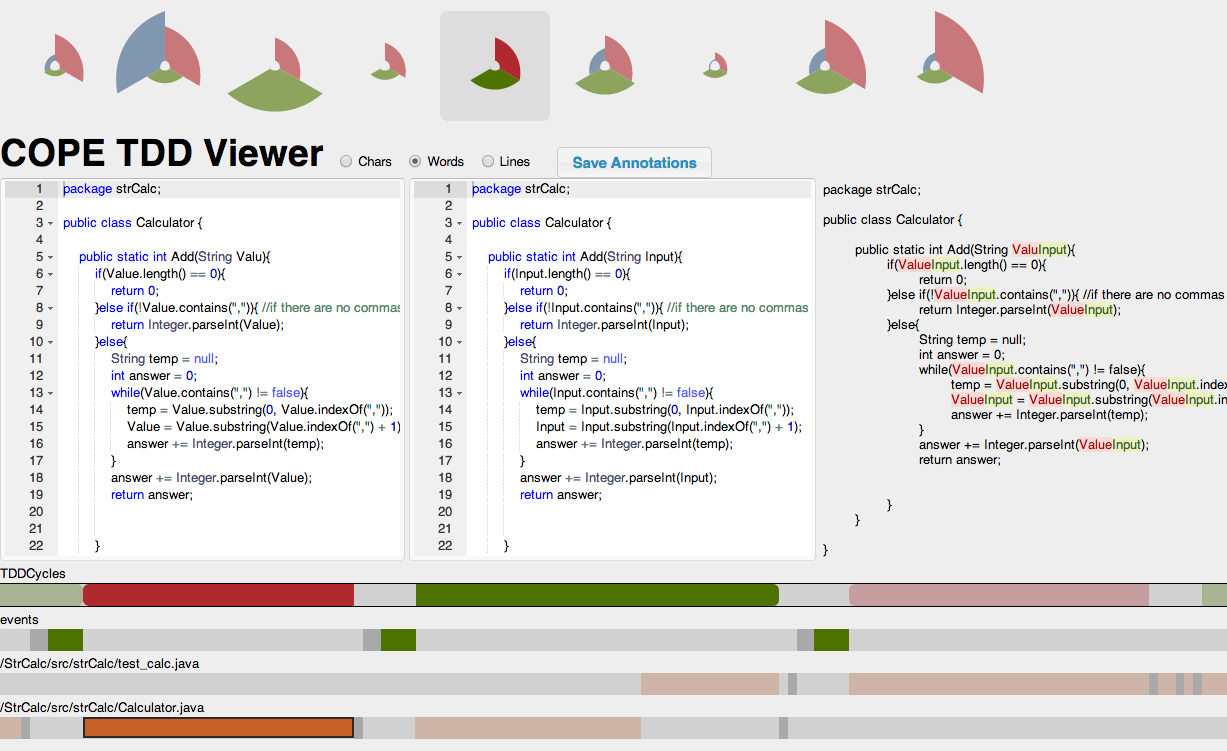
\includegraphics[width=\textwidth]{fig1}
	\caption{Overall view}
\label{fig:one}
\end{figure*}

The bottom bar shows the granular code changes via the TDD Atomic chart. It is also a navigational tool that users use to browse through events and view code diffs.
The mapping from the granular code changes to TDD stages is present via the top band which constitutes the TDD Spectrum chart.

In the middle there are three editors that show the code changes between two arbitrary text events in the TDD Atomic Chart. The first two editors show the first and the last variant of the code while the third editor shows the diff between the two: green highlights for added text and red highlights for deleted text.

\subsection{TDD Atomic Chart}
\label{sec:atomic}

\subsubsection{Justification}

This visualization allows the developer to navigate through the code events.
Each coding event is abstracted away via a rectangle. Moreover, the events are grouped by the files in which they are performed. The event rectangles are sorted via their timestamps. Temporal data abstraction and data clustering techniques from \cite{one} inspired this visualization: complex coding events are abstracted via rectangles and event types are clustered: event types are encoded via square color. A similar visualization is the Cluster Calendar View presented in \cite{one}.

The temporal succession of rectangles also provides the affordance of time flow. It resembles soundwave amplitude visualizations from sound editors and music players.
However, one key difference from a sound editor is that while the sound editor shows continuous data, we show cycle snapshots, so our visualization resembles more closely small multiples.
Lastly, the temporal succession is not relative to real time but relative to event ordering. Thus we obtain an ordering similar to lamport timestamps.

\subsubsection{Encoding}

We used Mackinlay's Ranking to assign encodings based on information ordering by importance.

The temporal succession of events (quantitative) is the most important invariant we wish to convey and thus we used position.
Next, we want to convey the event types (quantitative), for which we use color.

Events are grouped in several horizontal axis as following: 
\begin{itemize}
	\item The text events for each source file are shown in a separate axis.
	\item Text events from all other files and test events from source files are shown together in a common axis.
\end{itemize}
This grouping allows users to browse the events for a particular file and it also allows them to quickly spot the test events (highly relevant to TDD).

In order to alleviate the problem of having large amounts of data, we take advantage of the fact that text events come in bursts.
Thus, we detect the intermediary text events from inside the bursts and display them in a shortened manner.

\subsection{TDD Spectrum Chart}
\label{sec:spectrum}

\subsubsection{Justification}

The visualization in Figure~\ref{fig:two} enables developers, managers and researchers to answer many of their questions. It shows the succession of TDD stages in time and provides an intermediary mapping between high level TDD cycles and low level text events. 

Since users' main concern is the study of TDD, we chose to integrate this chart on top of the Atomic Chart.
This integration provides both a tight mapping to granular events and an intermediary transition to the high level Pulse chart as well.
Since the Spectrum chart is both close to and aligned with the Atomic chart, the users would tend to instinctively visually group code changes by TDD stage (gestalt principle: instinctively continuing an interrupted interval).

\begin{figure*}
	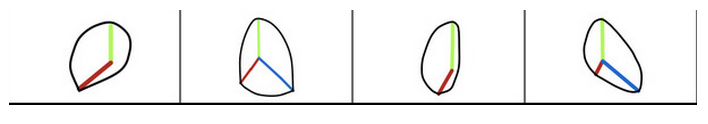
\includegraphics[width=\textwidth]{fig3.png}
	\caption{TDD Pulse Chart}
	\label{fig:three}
\end{figure*}

\begin{figure*}
	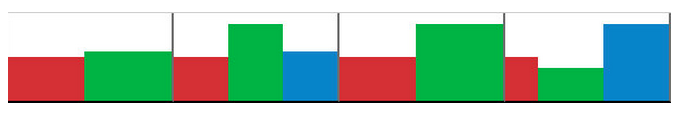
\includegraphics[width=\textwidth]{fig2.png}
	\caption{TDD Spectrum Chart}
	\label{fig:two}
\end{figure*}

\subsubsection{Encoding}

We ordered our encodings using Mackinlay's ranking.

Since the TDD cycle is defined by a temporal repetition of stages, the sequence of stages (categorical data) is encoded via position on the horizontal axis.
By doing so we also ensure a common axis with the Atomic chart.

The TDD stage type (categorical) is encoded via color: red for tests, green for development and blue for refactoring (colors are established by TDD literature). We chose color since position was taken by encoding temporal succession.

Cycle membership (categorical) is encoded via shape: the beginning and ending stages of the same cycle have rounded corners.
This makes the users intuitively split the stages by cycles since the rounded corners visually create partitions in the Spectrum chart.
We chose not to use higher ranked encodings (connection, containment, density) in Mackinlay's ranking because the stages are represented in a visually compact style and any other extra markings would have over-cluttered the chart.

\subsection{TDD Pulse Chart}
\label{sec:pulse}

\subsubsection{Justification}

The purpose of this visualization is to represent an entire TDD cycle by just one shape. 

By doing so, users obtain a singular mental image of an entire TDD cycle.
\cite{one} presents this technique as temporal data abstraction, in which complex, large temporal data is abstracted and mapped to qualitative entities, in our case, shape.

The visualization (figure~\ref{fig:three}) has its inspiration in the stacked hive plot.
Each TDD stage in the cycle is represented by a section of a disc.
The radius of the disc encodes a certain metric pertaining to that stage.

With this information the users can answer questions about what part of the TDD cycle they spend the most time on and how big their cycles are. They can also analyze how their cycles vary over time and whether any patterns occur.

Moreover, users can compare the TDD cycles for several users by showing several TDD time series side by side. This allows comparison of how much time different developers spend in stages, how big their stages are and whether they follow TDD at all.

\subsubsection{Encoding}

As with the timeseries chart, the sequence of TDD pulses are encoded via position, due to the temporal cyclic property of TDD cycles. We thus obtain small multiples snapshots of how the TDD cycle progresses in time.
TDD cycle metrics are encoded via the next available encoding, length (the radar chart axis).

%small and need to discern differences. The discs pop out, by growing in area
Since TDD cycles repeat themselves, the pulse chart would contain a series of small charts, each depicting a TDD cycle.
Therefore the main requirement that drove the design of this chart was the fact that it needed to be small and still intuitively convey information on the contents of a cycle.
Because TDD stage metrics are encoded in the radius of each disc section, increasing the radius increases the area by a power of 2.
Thus, small variations in metrics are visible to the user even if the chart is small.
Lastly, by using area, the chart utilizes as much empty space as possible.

%idea of a cycle
Another benefit of the pulse chart is that it expresses the idea of a repetitive event, a cycle.
This affords very well the nature of TDD cycles.

\subsection{Bidirectional mappings and user focus}

According to \cite{two}, visualization platforms do not only need to provide visualizations for several levels of abstraction but the different levels need to be in sync as well.
A selection in a particular visualization needs to propagate to the other visualizations as well.
Moreover, there must be visual cues that show the user's current focus.

%pulse to cycles (background select, scroll in cycle, select cycles, fade?)
%cycle to pulse (background select, scroll to pulse, select pulse, highlight cycle in pulse)
Our tool provides bidirectional navigation between TDD cycles and stages.
A selection of a TDD cycle in the Pulse chart causes an automatic selection of the corresponding stages in the Spectrum chart and a selection of a TDD stage in the Spectrum chart causes the automatic selection of its containing cycle in the Pulse chart.

Both charts visually mark their selections to provide cues of the user's current focus.
The selection in the Pulse chart is achieved by fading out unselected cycles and coloring the background of the selected one.
The selection in the Spectrum chart is achieved by fading out unselected stages.

%events - stages is automatically done by gest
The mapping between events in the Atomic chart and TDD stages in the Spectrum chart is intuitively achieved by the shared horizontal axis.

The Atomic chart also shows current user focus by fading out events that are not selected.
\section{Implementation}

Our tool is written in javascript.
Its implementation relies on various libraries.
The Pulse Chart is implemented in D3 \cite{three} and based on a Hive Chart \cite{four}.
We used the JSDiff library \cite{five} for diffing the code between different text events.

\begin{figure}
	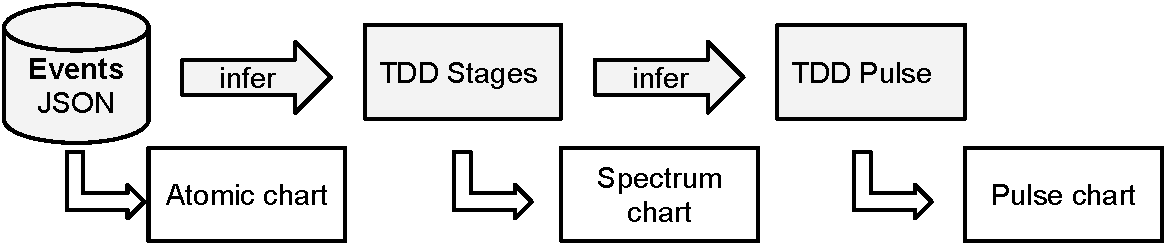
\includegraphics[width=\columnwidth]{implementation}
	\caption{TDD Viewer Pipeline}
	\label{fig:tool_pipeline}
\end{figure}

The overall pipeline data flow of our tool is depicted in figure \ref{fig:tool_pipeline}.

The input is a JSON file representing all the recorded fine grained events (see section \ref{sec:data} for event contents).
The fine grained events are graphically represented by the Atomic Chart (section \ref{sec:atomic}).

TDD stages are inferred from the recorded events.
Red, Green and Blue stages contain events recorded while writing the tests, making the tests pass and performing refactorings, respectively.
TDD stages are graphically represented via the Spectrum Chart (section \ref{sec:spectrum}).

The TDD pulse is inferred from the stream of TDD stages and the succession of pulses represents the practice of TDD.
A pulse contains a succession of red, green and blue stages.
While the red and green stages are mandatory, the blue stage is optional.
The TDD pulse is graphically represented by the Pulse Chart(section \ref{sec:pulse}).

\section{Usage scenarios}

Based on figure~\ref{fig:one} users can perform the following activities:
\begin{itemize}
	\item Analyze the pulse chart to answer their questions about TDD (section \ref{sec:highq}). 
	They can quickly detect any recurrent patterns, investigate how much code  they write in each phase (or how much time is spent) and judge on how close they are following TDD practices.
	
	\item They can explore the code changes for a certain cycle or stage. 
	Clicking on any item in the pulse chart the corresponding stages light up.
	Clicking on any text change event shows the code before and after the change, and the diff as well.
	
	\item Better define the TDD stages.
	Users can select any TDD stage in the Spectrum chart and resize it, to better account for the events that make part of it.
\end{itemize}

\subsection{Insights}

%Mackinlay's ordering does not always work. ex: cluttering
We found out that upholding Mackinlay's ranking does not lead to optimal results in some cases.
For example, our Spectrum chart has a compacted style and when encoding yet another piece of information (grouping stages by cycle) we had to skip several rankings (connection, containment) until we came to one that looked acceptable on our compact chart (area).

%Designing for small things
Designing for small sized charts brings a set of constraints to the design process.
For example, our pulse charts needed to fit in a 100 x 100 pixel square.
While we were trying different approaches, we observed that it was hard to discern small variations in data.
Therefore we opted to use encodings for the pulse chart that amplify small variations.
By encoding data in a disc section (defined by the radius), whenever the radius would change, the disc surface would change by a power of two, thus amplifying the small variation in the radius.

%iterations are quite good, no new news here
The iterative design process went very smooth for us.
Making small steps allowed us to avoid getting stuck.
For example, with the Pulse chart we went through about 4 or 5 variants until we settled on the petal like approach.

%the importance of preffering intuitive pre attentive cues rather than resorting to complex mental operations (tying by number, etc)

\section{Problems}

%lots of events
One of the problems that we faced (and still face) is the large volume of data that we have to deal with because our data includes many development events (each keystroke, eacy copy paste, each test, each lunch etc) we are.
We alleviated this issue by grouping the events by source file, adopting the soundwave metaphor and shrinking intermediary text changes.

%fake data
%not clean
Assigning low level events to TDD stages is a process that is currently done manually.
We have strived to provide intuitive fast means of creating and manipulating stages.

\section{Future work}

%compare with others
We intend to grow our tool to support the comparison of multiple developers' TDD practice, thus allowing the tool's users to answer all questions regarding developer comparison (section~\ref{sec:highq}).
A comparison page would contain multiple pulse charts, one for each developer (figure~).
Moreover, we can collapse a developer's cycles into a single pulse chart, thus facilitating comparison.


%selective events
In order to mitigate the problem of having a large volume of data, we plan to allow the user to choose which events to display.
Another approach would be to show only the events pertaining to a cycle, when a cycle is selected.

%automatic detection of 
Currently users have to manually define the TDD stages.
We would design an algorithm that automatically bins detects TDD stages.
 
%% if specified like this the section will be committed in review mode
%\acknowledgments{}

\bibliographystyle{abbrv}
%%use following if all content of bibtex file should be shown
%\nocite{*}
\bibliography{design-pass-1}
\end{document}

